\documentclass[conf]{new-aiaa}
%\documentclass[journal]{new-aiaa} for journal papers
\usepackage[utf8]{inputenc}

\usepackage{graphicx}
\usepackage{amsmath}
\usepackage[version=4]{mhchem}
\usepackage{siunitx}
\usepackage{longtable,tabularx}
\setlength\LTleft{0pt} 

\title{Enhancing large eddy simulation sub-grid scale closure model estimation using Convolutional Neural Networks}

\author{K. Liu\footnote{Undergraduate, Department of Mechanical and Aerospace Engineering, kliu0036@student.monash.edu}, J. Soria\footnote{Deputy Head, Department of Mechanical and Aerospace Engineering, julio.soria@monash.edu}}
\affil{Monash University, Melbourne, Victoria, 3800, Australia}

\begin{document}
% \spacing{2}
\maketitle

\begin{abstract}
    In large eddy simulations (LES), the primary challenge is the development of a robust sub-grid scale closure model. Utilising the recent developments of specialised machine learning (ML) algorithms in various data driven applications, this paper reports on the implementation of a Convolutional Neural Network (CNN) trained a priori using course grid field data to serve a posteriori as an alternative to existing physics-based closure models. To this end, Direct Numerical Simulation (DNS) of 2D decaying homogeneous isotropic turbulence (2D-DHIT) at a Reynolds Number of up to 32,000 has been conducted based on a dimensionless vorticity-streamfunction form using a pseudo spectral method on a 2048 x 2048 grid. A Gaussian filter was employed to compute the coarse-grid vorticity, streamfunction, as well as the sub-grid scale (SGS) terms, which were saved at periodic intervals and served as high-fidelity training data for the CNN. The CNN was trained from multiple independent DNS runs where the optimal CNN parameter values saved and subsequently used online as the SGS model during LES. Benchmarking of the LES performance against the filtered DNS data in terms of turbulent kinetic energy (TKE) spectra and vorticity probability density functions (PDF) is undertaken and is reported and discussed.
\end{abstract}

\section*{Nomenclature}

{\renewcommand\arraystretch{1.0}
\noindent\begin{longtable*}{@{}l @{\quad=\quad} l@{}}
$c$ & Correlation coefficient\\
$E(k)$ & Turbulent kinetic energy\\
$G$ & Gaussian filter \\
$\mathbf{i}$ & Complex unit \\
$i$  & x index \\
$j$  & y index \\
$\mathbf{k}$  & Wavenumber (vector) \\
$k$  & Wavenumber \\
$l_{v}$ & Enstrophy dissipation scale \\
$m$ & k-space x index \\
$n$ & k-space y index \\
$\mathcal{N}$ & Nonlinear advection operator \\
$N_{x},N_{y}$ & gridpoints in (x,y) \\
$Re$ & Reynolds number \\
$\Delta$ & Discrete grid spacing\\
$\Delta_{F}$ & Filter width\\
$\Delta t$ & Time step \\
$\Pi$ & SGS model \\
$\eta$ & Kolmogorov length scale\\
$\sigma$ & Standard deviation \\
$\psi$ & Streamfunction \\
$\omega$ & Vorticity \\
$\overline{(\cdot)}$ & Filtered variable\\
$\tilde{(\cdot)}$ & Fourier transformed variable
\end{longtable*}}
\section{Introduction}
\lettrine{T}{o} this day, turbulence remains one of the greatest unsolved problems in physics, as certain quantities in turbulent fluid flow can be both difficult to measure experimentally and model computationally due to their chaotic nature. In the context of turbulent flow, the governing partial differential equations (PDEs) are the 2D Navier-Stokes equations (NSEs), which are formulated in vorticity-streamfunction form. The scenario investigated in this work is that of 2D decaying homogeneous isotropic turbulence (2D-DHIT), which is found largely on the scale of geophysical and environmental flows, and is commonly used as a testbed for machine learning (ML) based techniques for SGS modelling\cite{xie2019artificial,2022_LES_CNN,TABELING20021,vallis2017atmospheric}.
\par 
In direct numerical simulation (DNS), all relevant spatial and temporal scales must be directly solved\cite{moin1998direct}, which may span several orders of magnitude between the domain length and Kolmogorov scale. This is exemplified by the relationship between the computational cost of DNS and Reynolds Number, which scales at the order of $O(Re^{3})$ in 3D\cite{DNS1970}. Therefore, resolving turbulent flows using DNS is very expensive computationally, making it infeasible for most real-world applications. Large eddy simulations (LESs) circumvent this by only resolving the flow at scales larger than the grid size, and applying a model to correctly capture the subgrid scale (SGS) effects\cite{pope2000turbulent}, striking a balance between accuracy and performance. Therefore, the accuracy of LES solutions is strongly dependent on the validity of the SGS model, where the development of an accurate model has been an active area of research for the past half century. 
\par
Machine learning (ML) has been widely used in areas such as image and speech recognition, cognitive science, and genomics due to the recent abundance of available training data and increase in computational power\cite{Raissi_part1}.
Using ML, the SGS terms in LES may instead be predicted non-parametrically by giving it only data at the resolved scale. There has been work done in the past few years using fully connected artificial neural networks (ANNs) which aim to locally estimate the SGS term using nearby grid points, as performed by \citeauthor{maulik2019subgrid} \cite{maulik2019subgrid} for the same scenario of 2D-DHIT. Here, we aim globally estimate the SGS terms which will be done using a CNN.
CNNs are a form of neural network commonly found in computer vision and image processing applications as they work well with spatial data. This feature of CNNs translates well to the task of SGS terms, as the fluid flow is highly dependent on spatial features. 


 
\section{Methodology}
\subsection{DNS and LES}
\subsubsection{Governing equations}
The equations governing the 2D-DHIT is the dimensionless vorticity-streamfunction ($\omega$ - $\psi$) formulation of the NSEs, which are defined as:
\begin{subequations}
    \label{NSEs}
    \begin{gather}
        \frac{\partial \omega}{\partial t} + \mathcal{N}(\omega,\psi)=\frac{1}{Re}\nabla^{2}\omega   \label{eq:vort}\\ 
        \nabla^{2}\psi=-\omega \label{eq:streamvort}
    \end{gather}
\end{subequations}
where $\mathcal{N}(\omega,\psi)$, the nonlinear advection term, is given by:
\begin{equation}
    \label{nonlinearphys}
    \mathcal{N}(\omega,\psi) = \frac{\partial \psi}{\partial y}\frac{\partial \omega}{\partial x}-\frac{\partial \psi}{\partial x}\frac{\partial \omega}{\partial y}
\end{equation}
The main advantage of formulating the NSEs in $\omega$ - $\psi$ form is the elimination of pressure as a variable by virtue of it being a conservative field. The divergence-free condition is also automatically satisfied, with the streamfunction poisson equation \eqref{eq:streamvort} taking its place. 

Once the filtering operation $\overline{(\cdot)}$ has been applied, we obtain our equations for LES:
\begin{subequations}
    \begin{gather}
        \frac{\partial \overline{\omega}}{\partial t} + \mathcal{N}(\overline{\omega},\overline{\psi})=\frac{1}{Re}\nabla^{2}\overline{\omega}+\Pi\\
        \nabla^{2}\overline{\psi}=-\overline{\omega}
    \end{gather}
\end{subequations}
with our SGS term $\Pi$ being defined as:
\begin{equation}
    \Pi = \mathcal{N}(\overline{\omega},\overline{\psi})-\overline{\mathcal{N}(\omega,\psi)}
\end{equation}
For the filtering operation, the Gaussian filter was chosen as it is compact in both physical and k-space \cite{2022_LES_CNN,pope2000turbulent}. The filter kernel is defined as the following:
\begin{equation}
    G = \exp (- {| \mathbf{k}_{DNS}\vert}^2 {\Delta}^2_{F} /24)
\end{equation}
Where the filter width ${\Delta}_{F}$ is defined to be twice the size of the LES grid spacing (${\Delta}_{LES}$) to ensure sufficient grid spacing \cite{pope2000turbulent}.
In order to apply the filtering operation, elementwise multiplication is applied between the kernel and the quantity of interest in k-space. Using vorticity as an example, the filtered variable is obtained from the operation:
\begin{equation}
   \overline{\tilde{\omega}} = G \odot \tilde{\omega}
\end{equation}
After the solution is transferred to the coarser LES grid, wavenumbers whose combined x-y magnitude is past the cutoff as defined by $k_{c} = \sqrt{2}\pi /{\Delta}_{LES} $ are discarded. 

\subsubsection{Numerical method}
For the remainder of this paper, we will exclusively analyse 2D-DHIT at a $Re$ of 32000. The spatial resolution $(N_{x},N_{y})$ at which equations \eqref{NSEs} will be solved using DNS is 2048 by 2048. Given a doubly periodic square domain of [0,$2\pi$] $\times$ [0,$2\pi$], the grid spacing is defined as $\Delta_{DNS} = \frac{2\pi}{N}$ where $N$ is the number of gridpoints. The DNS runs are fully resolved as $k_{max}l_{v}\geq 3.0$ and $k_{max}\eta \geq 1.5$, where $k_{max}$ is the maximum Fourier wavenumber\cite{kmax_fullresolve}. The time step used is $\Delta t=10^{-4}$ and the DNS will be run from $t=0.0$ to $t=4.0$, requiring 40000 time steps. Initial conditions are generated as a random vorticity field with identical according to the method described in the appendix, where the randomly generated vorticity field will always have the same TKE spectrum. The LES has a grid size of 256 by 256 and a time step of $\Delta t_{LES}=10^{-3}$, resulting in 640 times fewer degrees of freedom compared to the DNS.

The pseudospectral method is naturally the most ideal way to solve equations \eqref{eq:vort} and \eqref{eq:streamvort} given uniform grid spacing and periodic boundary conditions. The discrete Fourier transform (DFT) takes a variable $u_{i,j}$ and transforms it into $\tilde{u}_{m,n}$ as defined in k-space. Given a set of $N_{x}\times N_{y}$ equidistant points on the interval [0,$2\pi$] $\times$ [0,$2\pi$], the DFT on a spatial variable a variable $u_{i,j}$ is \cite{DNS_Primer,Python_spectral}:
\begin{equation}
    \label{FFT}
    u_{i,j} = \sum_{m = -\frac{N_{x}}{2}}^{\frac{N_{x}}{2}-1}\sum_{n = -\frac{N_{y}}{2}}^{\frac{N_{y}}{2}-1} \tilde{u}_{m,n}\exp (\mathbf{i}(k_{x}x_{i}+k_{y}y_{j}))
\end{equation}
and the inverse transform is
\begin{equation}
    \label{inverseFFT}
    \tilde{u}_{m,n} = \frac{1}{N_{x}N_{y}}\sum_{i=0}^{N_{x}-1}\sum_{j=0}^{N_{y}-1} u_{i,j}\exp (-\mathbf{i}(k_{x}x_{i}+k_{y}y_{j}))
\end{equation}
where ($x_{i},y_{j}$) and ($k_{x},k_{y}$) represent the discrete spatial coordinates and wavenumbers respectively.

In k-space, it is possible to achieve exponential "infinite order" truncation error far below machine epsilon \cite{DNS_Primer} compared to polynomial truncation error found in finite difference schemes. By exploiting symmetry, the FFT algorithm can perform a discrete Fourier transform in $O(Nlog(N))$ operations, scaling favourably with large problems \cite{cooley1965algorithm}. In k-space, equations \eqref{eq:vort} and \eqref{eq:streamvort} become:
\begin{subequations}
    \begin{gather}
        \frac{\partial \tilde{\omega}}{\partial t} + \mathcal{\tilde{N}}(\tilde{\omega},\tilde{\psi})=\frac{-1}{Re}(k_{x}^{2}+k_{y}^{2})\tilde{\omega}   \label{eq:vort_wave}\\ 
        (k_{x}^{2}+k_{y}^{2})\tilde{\psi}=\tilde{\omega} \label{eq:streamvort_wave}
    \end{gather}
\end{subequations}
where the nonlinear advection term becomes the following convolution
\begin{equation}
    \label{nonlinearwave}
    \mathcal{\tilde{N}}(\tilde{\omega},\tilde{\psi}) = (\mathbf{i}k_{y}\tilde{\psi})\ast (\mathbf{i}k_{x}\tilde{\omega})-(\mathbf{i}k_{x}\tilde{\psi})\ast (\mathbf{i}k_{y}\tilde{\omega})
\end{equation}
The nonlinear term is evaluated in physical space, where after an inverse FFT operation, the convolution terms become multiplication and we obtain equation \eqref{nonlinearphys}.
To obtain the streamfunction from the vorticity field, equation \eqref{eq:streamvort} can be solved using a fast Poisson solver (FPS) consisting of the following steps:
\begin{enumerate}
    \item Transform variables into k-space using FFT
    \item Calculate streamfunction coefficients in the following manner
    \begin{equation*}
        \tilde{\psi} = \frac{\tilde{\omega}}{(k_{x}^{2}+k_{y}^{2})}
    \end{equation*}
    \item Use the inverse transform described by equation \eqref{inverseFFT}.
\end{enumerate}
When performing FFTs to solve the nonlinear term, one must deal with aliasing errors that arise from the multiplication of Fourier coefficients resulting in a wavenumber larger than what could be represented on the discrete grid \cite{Orszag_Alias,pope2000turbulent}. This aliasing error must be accounted for, as it contaminates the large physical scales and could potentially cause the solution to blow up, requiring additional viscosity to dampen these errors \cite{Bowman_dealias,Phillips1959}. The aliasing error is removed completely by using the 3/2 zero padding technique, where the array of Fourier coefficients is increased by a factor of 3/2 and populated with zeroes \cite{Python_spectral,Bowman_dealias,Orszag_Alias}.

To step forward in time, a hybrid third order Runge-Kutta and Crank-Nicolson (RK3-CN) as described by \citeauthor{RK3CN} in Fluid Flow Phenomena: A Numerical Toolkit \cite{RK3CN} was used. The scheme is third order accurate and explicit in time for the nonlinear component, but second order accurate and implicit for the linear diffusion component. Applied to equation \eqref{eq:vort_wave}, the RK3-CN algorithm is:
\begin{equation}
    \begin{aligned}
        \tilde{\omega}' &= \tilde{\omega}^{n} + \Delta t(\gamma_{1}\tilde{\mathcal{N}}^{n} + \rho_{1}\tilde{\mathcal{N}}^{(n-1)''} - \alpha_{1} \left(\frac{k_{x}^{2}+k_{y}^{2}}{2Re}\right)(\tilde{\omega}'+\tilde{\omega}^{n}))\\
        \tilde{\omega}'' &= \tilde{\omega}' + \Delta t(\gamma_{2}\tilde{\mathcal{N}}' + \rho_{2}\tilde{\mathcal{N}}^{n} - \alpha_{2} \left(\frac{k_{x}^{2}+k_{y}^{2}}{2Re}\right)(\tilde{\omega}''+\tilde{\omega}'))\\
        \tilde{\omega}^{n+1} &= \tilde{\omega}'' + \Delta t(\gamma_{3}\tilde{\mathcal{N}}'' + \rho_{3}\tilde{\mathcal{N}}' - \alpha_{3} \left(\frac{k_{x}^{2}+k_{y}^{2}}{2Re}\right)(\tilde{\omega}^{n+1}+\tilde{\omega}''))
    \end{aligned}
\end{equation}
Where the nonlinear term $\tilde{\mathcal{N}}$ is given by equation \eqref{nonlinearwave} and is evaluated by the quantities $\tilde{\omega}$ and $\tilde{\psi}$ at the respective timestep. The coefficients $\gamma, \rho, \alpha$ used in the RK3-CN scheme are:
\begin{align*}
    \gamma_{1} &= -8/15 & \rho_{1} &= 0 & \alpha_{1} &= 8/15\\
    \gamma_{2} &= -5/12 & \rho_{2} &= 17/60 & \alpha_{2} &= 2/15\\
    \gamma_{3} &= -3/4 & \rho_{3} &= 5/12 & \alpha_{3} &= 1/3
\end{align*}
This scheme was chosen as it is superior to the commonly used Adams-Bashforth 2 (AB2) scheme. RK3-CN is stable for CFL numbers up to $\sqrt{3}$ compared to 1 for AB2, which is important as transient shocks during the flow evolution can magnify the local CFL number \cite{RK3CN}.

\subsection{Training CNN}
A CNN was constructed with 10 pure convolution layers (no pooling or upsampling) with 64 channels each with a 5$\times$5 kernel size. The activation function chosen was the rectified linear function (ReLu) except for the last output layer, which was a one to one map.
The inputs to the CNN are the global filtered vorticity and streamfunction fields, and the output is the SGS term. As is best practice in machine learning, the training samples are normalised to their individual standard deviations \cite{MLstandardise}. Mathematically, our CNN model is represented as an optimal map $\mathbb{M} $ between the inputs and outputs:
\begin{equation}
    \mathbb{M} : {\{ \overline{\psi}/\sigma_{\overline{\psi}},\overline{\omega}/\sigma_{\overline{\omega}}\}\in \mathbb{R}^{2\times N_{LES}\times N_{LES}} \rightarrow \{ \overline{\Pi}/\sigma_{\overline{\Pi}}\}\in \mathbb{R}^{1\times N_{LES}\times N_{LES}}}
\end{equation}
The objective function for the model to minimise is the mean squared error (MSE) 
\begin{equation}
    MSE = \frac{1}{n}\sum_{i = 1}^{n}\left\lVert \Pi^{CNN}_{i} - \Pi^{FDNS}_{i} \right\rVert ^{2}
\end{equation}
The optimisation algorithm used was ADAM with a learning rate of 1e-5, a first-order gradient based optimisation algorithm \cite{ADAM}. As the total training data pool was far too large to be trained at once, minibatches of 40 samples were used to train the CNN. Given a total of 18000 training samples, 450 iterations were required to complete a single epoch (complete pass of the dataset). Training data for the CNN is taken from the DNS run after the flow exhibits self-similarity. To verify the performance of the CNN model, the correlation coefficient between the test data SGS terms and those predicted by the CNN will be recorded. The correlation coefficient $c$ is defined as:
\begin{equation}
    c = \frac{Cov(\Pi^{CNN},\Pi^{FDNS})}{\sigma_{\Pi^{CNN}}\sigma_{\Pi^{FDNS}}}
\end{equation}
The test data has 300 samples and is taken from an independent DNS run which is not seen at all by the CNN during training.
\section{Results}

\subsection{DNS results}
Regions which have positive vorticity are shaded red in figure \ref{fig:DNS_field} and cause the fluid domain to rotate anti-clockwise. Likewise, the opposite is true for negative vorticity regions which are shaded blue.
\begin{figure}[htp]
    \centering
    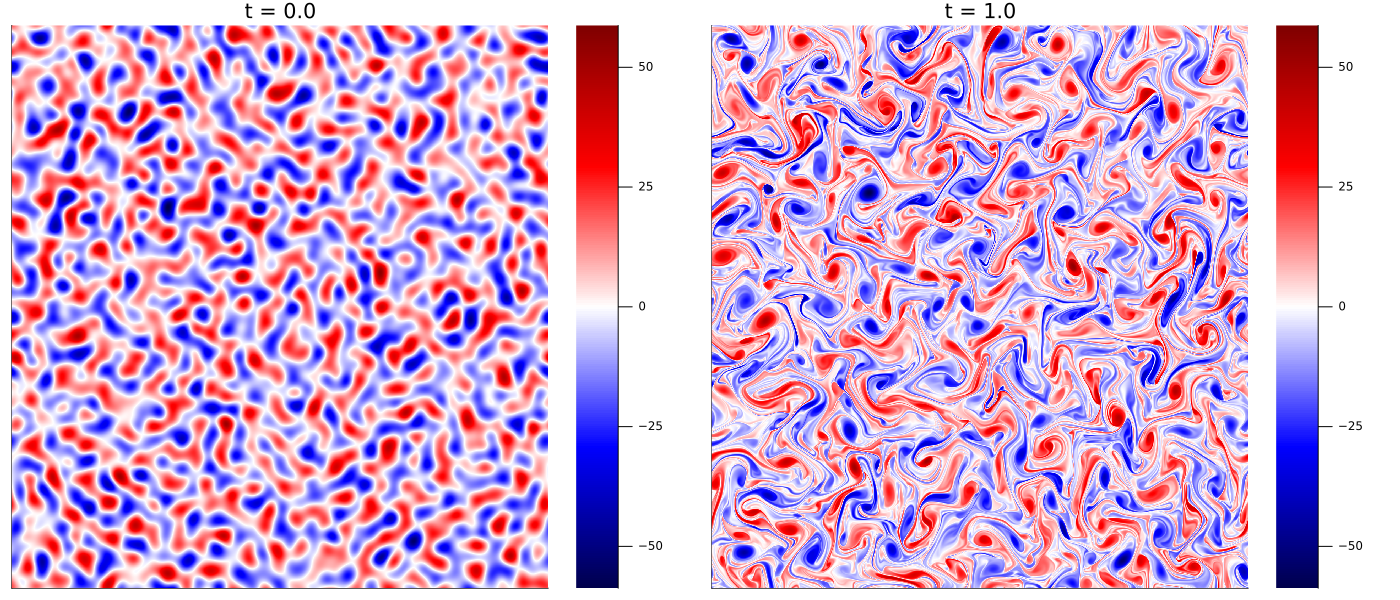
\includegraphics[width=0.8\textwidth]{DNS_field_1.png}
    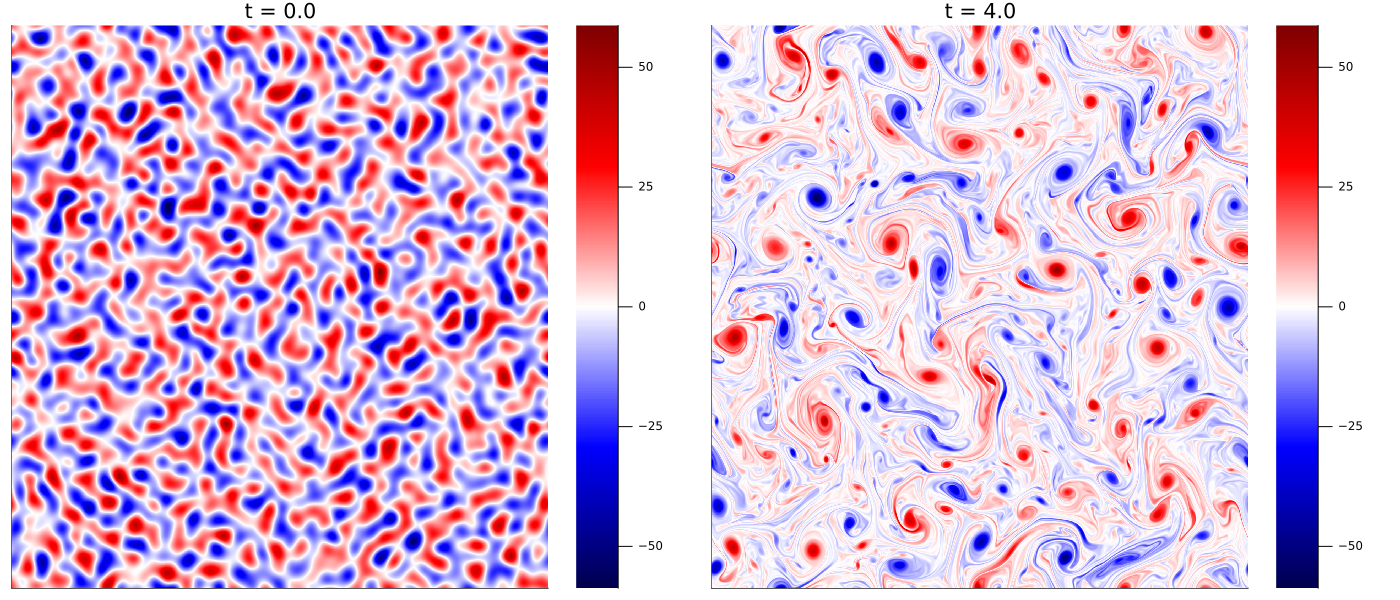
\includegraphics[width=0.8\textwidth]{DNS_field_4.png}
    \caption{Vorticity field of the 2D-DHIT at Re = 32000. Self-similarity begins at t=1.0 and simulation ends at t=4.0}
    \label{fig:DNS_field}
\end{figure}
\begin{figure}[htp]
    \centering
    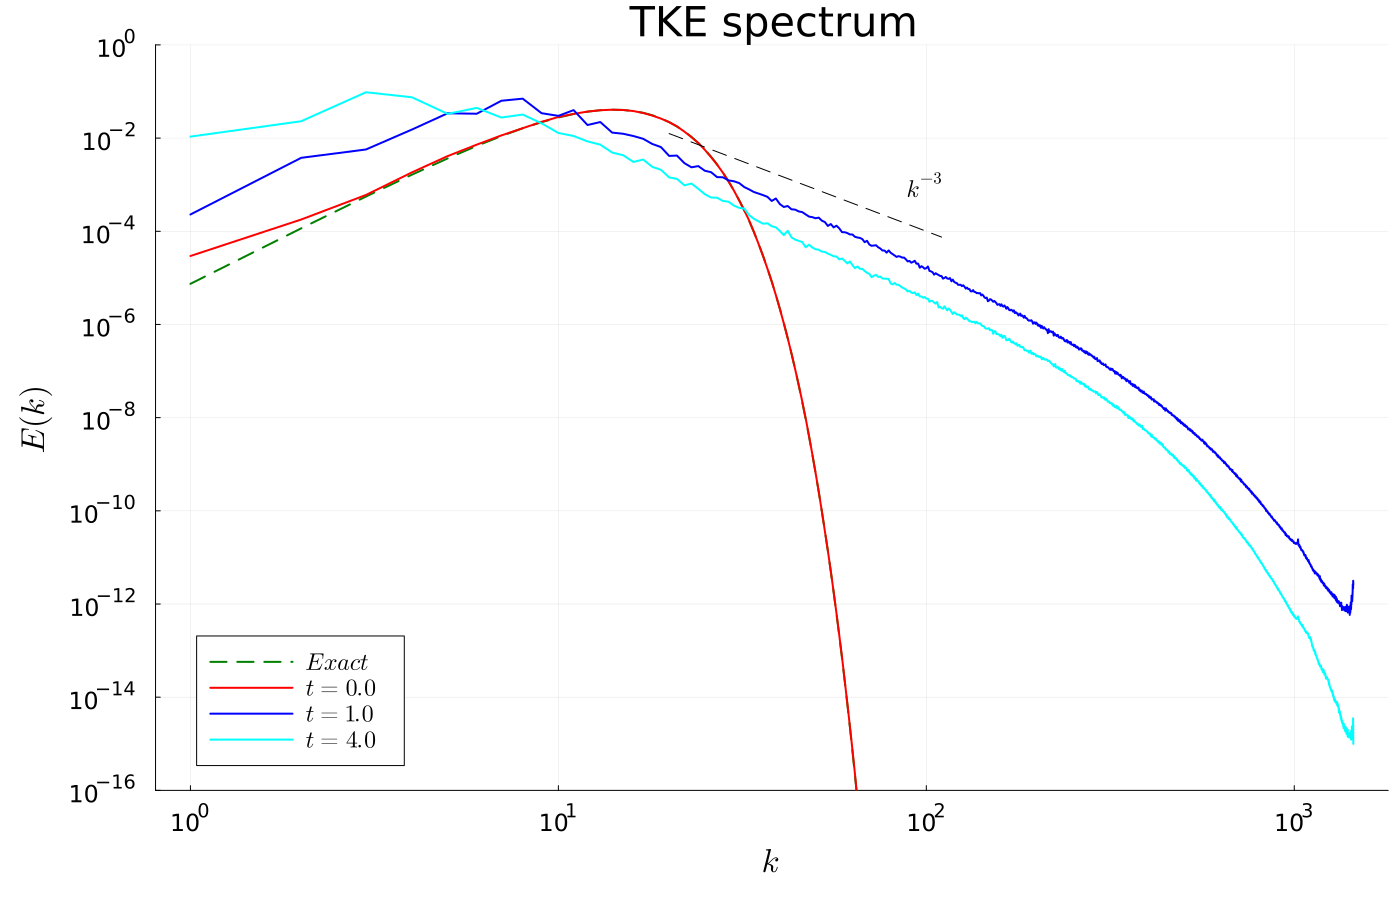
\includegraphics[width=0.8\textwidth]{TKE_1.png}
    \caption{Turbulent kinetic energy spectrum. The Initial energy distribution is overlaid with the analytical equation and the inertial subrange as predicted in \cite{Kraichnan,batchelor1969computation,leith1971atmospheric} is clearly seen after t = 1.0}
    \label{fig:TKE_1}
\end{figure}
After around $t=1.0$, the TKE spectrum begins to exhibit self-similarity, where an inertial range develops that follows the $k^{-3}$ scaling as theorised by Kraichnan-Batchelor-Leith \cite{Kraichnan,batchelor1969computation,leith1971atmospheric}.
\pagebreak
\subsection{A priori CNN}
After training on the dataset for over 60 epochs, the CNN reached a correlation coefficient of 0.81 with the test dataset. This outperforms physics based SGS models such as Smagorinsky \cite{2022_LES_CNN,pawar2020priori} which typically achieves a correlation coefficient of 0.55 as it is a purely diffusive model.
\pagebreak
\subsection{A posteriori CNN}
To run the CNN model a posteriori in a live CNN run, it must be scaled by the standard deviation of the SGS terms obtained from the DNS run. This is a consequence of input/output normalised training, where information on the standard deviation is lost. To remedy this, the ensemble average of the standard deviation of the SGS term was calculated at every time step, which is then used to renormalise the output of the CNN model.
\begin{figure}[h]
    \centering
    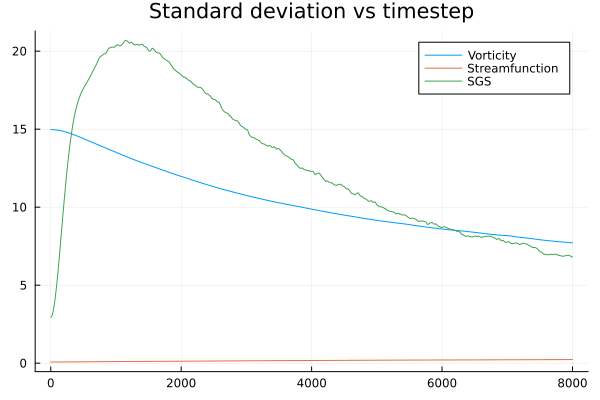
\includegraphics[width=0.75\textwidth]{STDs.png}
    \caption{The standard deviation for the SGS terms rises sharply before decaying.}
\end{figure}
The peak of the SGS term standard deviation occurs right before the onset of self-similarity, suggesting that eddies at scales below the LES grid are most prevalent shortly after the initial condition.

\pagebreak
\section{Conclusion}


\section*{Appendix A}
\label{appendix:A}

An Appendix, if needed, should appear before the acknowledgments.

\section*{Acknowledgments}

\bibliography{references}

\end{document}